% P08-F03 universal preprocessing renderer output -- copied estimates only
%% source SHA256: 8c910290a3d09cbc9f03e7dcde77ae1598487533b0c68cfa1709a42e7d38621d
%% semantic SHA256: 7045e1dc2788300144330414456a5725a0e4cd3af23681b05b2c9e546cf3b73c
\documentclass[border=0pt]{standalone}
\usepackage[T1]{fontenc}
\usepackage[utf8]{inputenc}
\usepackage{lmodern}
\usepackage{tikz}
\usepackage{pgfplots}
\pgfplotsset{compat=1.18}
\definecolor{PolA}{HTML}{0072B2}
\pgfplotsset{pt0/.style={only marks, mark=*, color=PolA, mark options={fill=PolA, draw=black}}}
\pgfplotsset{bar0/.style={PolA, line width=0.8pt, mark=|, mark options={color=PolA}}}
\definecolor{PolB}{HTML}{D55E00}
\pgfplotsset{pt1/.style={only marks, mark=square*, color=PolB, mark options={fill=PolB, draw=black}}}
\pgfplotsset{bar1/.style={PolB, line width=0.8pt, mark=|, mark options={color=PolB}}}
\pgfplotsset{domainpts/.style={only marks, mark=o, mark options={draw=gray, fill=none, scale=0.7}}}
\tikzset{intervalna/.style={font=\fontsize{8}{10}\selectfont, anchor=east}}
\begin{document}
\begin{minipage}{181.86mm}\centering
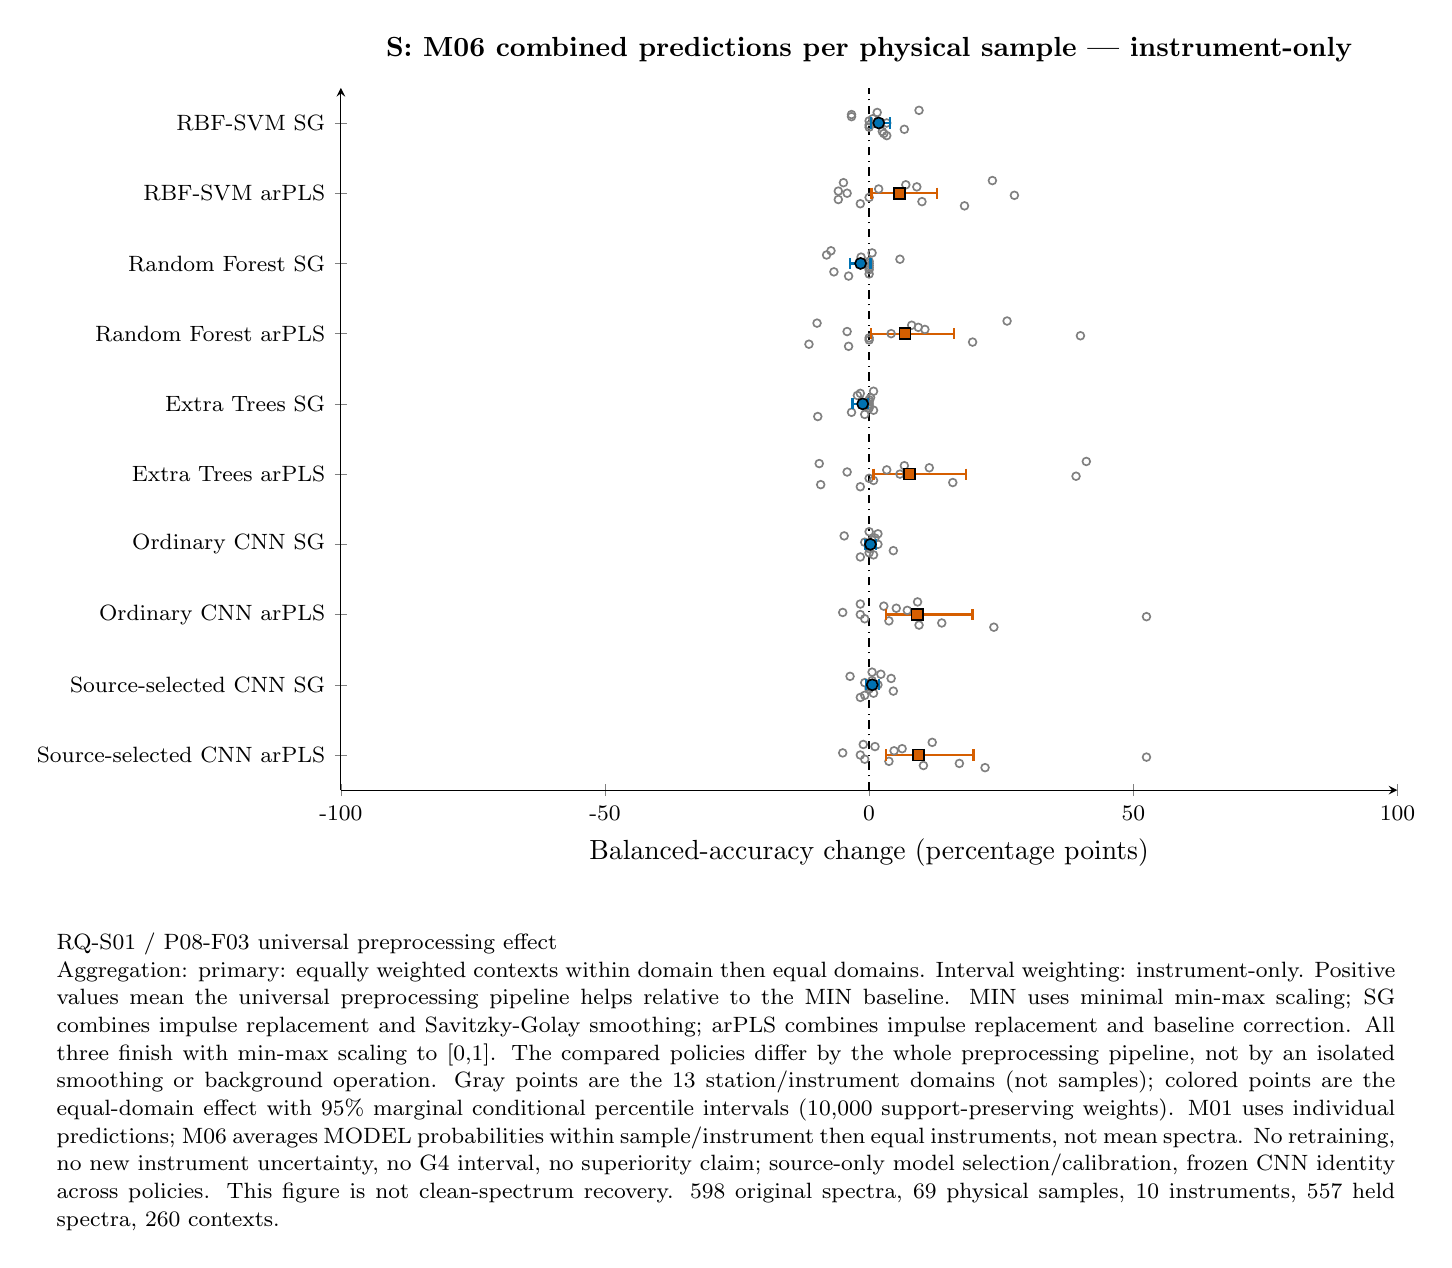
\begin{tikzpicture}
\begin{axis}[width=150mm, height=105mm, clip=false, xmin=-1, xmax=1, xtick={-1,-0.5,0,0.5,1}, xticklabels={-100,-50,0,50,100}, xlabel={Balanced-accuracy change (percentage points)}, ymin=-0.5, ymax=9.5, ytick={0,1,2,3,4,5,6,7,8,9}, yticklabels={{Source-selected CNN arPLS}, {Source-selected CNN SG}, {Ordinary CNN arPLS}, {Ordinary CNN SG}, {Extra Trees arPLS}, {Extra Trees SG}, {Random Forest arPLS}, {Random Forest SG}, {RBF-SVM arPLS}, {RBF-SVM SG}}, yticklabel style={font=\fontsize{8}{10}\selectfont}, tick label style={font=\fontsize{8}{10}\selectfont}, axis lines=left, title={S: M06 combined predictions per physical sample | instrument-only}, title style={font=\bfseries\fontsize{10}{12}\selectfont}, every axis plot/.append style={line width=0.6pt}]
\draw[black, dash dot, line width=0.6pt] (axis cs:0,-0.5) -- (axis cs:0,9.5);
\addplot[domainpts] coordinates {(0.03333333333333334,8.8200000000000003) (0.02777777777777778,8.8499999999999996) (0.025000000000000001,8.8800000000000008) (0.066666666666666666,8.9100000000000001) (0,8.9399999999999995) (0,8.9700000000000006) (0.033333333333333333,9) (0,9.0299999999999994) (0.0069444444444444449,9.0600000000000005) (-0.033333333333333333,9.0899999999999999) (-0.033333333333333333,9.1199999999999992) (0.015277777777777776,9.1500000000000004) (0.094444444444444442,9.1799999999999997)};
\addplot[bar0] coordinates {(0.0034159665025402935,9) (0.038765005071708832,9)};
\addplot[pt0] coordinates {(0.01816239316239316,9)};
\addplot[domainpts] coordinates {(0.18055555555555552,7.8200000000000003) (-0.01666666666666667,7.8499999999999996) (0.10000000000000001,7.8799999999999999) (-0.058333333333333334,7.9100000000000001) (0,7.9400000000000004) (0.27500000000000002,7.9699999999999998) (-0.041666666666666664,8) (-0.058333333333333327,8.0299999999999994) (0.018055555555555564,8.0600000000000005) (0.090277777777777804,8.0899999999999999) (0.069444444444444448,8.1199999999999992) (-0.048611111111111119,8.1500000000000004) (0.23333333333333334,8.1799999999999997)};
\addplot[bar1] coordinates {(0.0043786270836592587,8) (0.12873104912725802,8)};
\addplot[pt1] coordinates {(0.057158119658119663,8)};
\addplot[domainpts] coordinates {(-0.038888888888888883,6.8200000000000003) (0,6.8499999999999996) (-0.066666666666666666,6.8799999999999999) (0,6.9100000000000001) (0,6.9400000000000004) (0,6.9699999999999998) (0,7) (0,7.0300000000000002) (0.058333333333333334,7.0599999999999996) (-0.015277777777777779,7.0899999999999999) (-0.080555555555555533,7.1200000000000001) (0.0055555555555555549,7.1500000000000004) (-0.072222222222222215,7.1799999999999997)};
\addplot[bar0] coordinates {(-0.035827247354554122,7) (0.0026028994460529338,7)};
\addplot[pt0] coordinates {(-0.016132478632478631,7)};
\addplot[domainpts] coordinates {(-0.038888888888888883,5.8200000000000003) (-0.11388888888888889,5.8499999999999996) (0.1958333333333333,5.8799999999999999) (0,5.9100000000000001) (0,5.9400000000000004) (0.40000000000000002,5.9699999999999998) (0.041666666666666664,6) (-0.041666666666666664,6.0300000000000002) (0.10555555555555556,6.0599999999999996) (0.093055555555555558,6.0899999999999999) (0.080555555555555561,6.1200000000000001) (-0.098611111111111094,6.1500000000000004) (0.26111111111111113,6.1799999999999997)};
\addplot[bar1] coordinates {(0.0034371165272782315,6) (0.16041761125378307,6)};
\addplot[pt1] coordinates {(0.068055555555555564,6)};
\addplot[domainpts] coordinates {(-0.09722222222222221,4.8200000000000003) (-0.0083333333333333332,4.8499999999999996) (-0.03333333333333334,4.8799999999999999) (0.0083333333333333332,4.9100000000000001) (0,4.9400000000000004) (0,4.9699999999999998) (0,5) (0,5.0300000000000002) (0,5.0599999999999996) (0.0027777777777777792,5.0899999999999999) (-0.022222222222222223,5.1200000000000001) (-0.016666666666666666,5.1500000000000004) (0.0083333333333333332,5.1799999999999997)};
\addplot[bar0] coordinates {(-0.031374797294294779,5) (-0.0018788452240054564,5)};
\addplot[pt0] coordinates {(-0.01217948717948718,5)};
\addplot[domainpts] coordinates {(-0.016666666666666666,3.8199999999999998) (-0.091666666666666674,3.8500000000000001) (0.15833333333333333,3.8799999999999999) (0.0083333333333333332,3.9100000000000001) (0,3.9399999999999999) (0.39166666666666672,3.9700000000000002) (0.058333333333333334,4) (-0.041666666666666664,4.0300000000000002) (0.033333333333333333,4.0599999999999996) (0.11388888888888889,4.0899999999999999) (0.06666666666666668,4.1200000000000001) (-0.094444444444444428,4.1500000000000004) (0.41111111111111109,4.1799999999999997)};
\addplot[bar1] coordinates {(0.008296080380974933,4) (0.18410425760993213,4)};
\addplot[pt1] coordinates {(0.076709401709401714,4)};
\addplot[domainpts] coordinates {(-0.016666666666666666,2.8199999999999998) (0.0083333333333333332,2.8500000000000001) (0,2.8799999999999999) (0.045833333333333337,2.9100000000000001) (0,2.9399999999999999) (0,2.9700000000000002) (0.016666666666666666,3) (-0.0083333333333333332,3.0299999999999998) (0.0055555555555555549,3.0600000000000001) (0.01111111111111111,3.0899999999999999) (-0.047222222222222214,3.1200000000000001) (0.016666666666666666,3.1499999999999999) (-1.3877787807814458e-18,3.1800000000000002)};
\addplot[bar0] coordinates {(-0.0066766768226773649,3) (0.013254118540508539,3)};
\addplot[pt0] coordinates {(0.0024572649572649581,3)};
\addplot[domainpts] coordinates {(0.2361111111111111,1.8200000000000001) (0.094444444444444456,1.8500000000000001) (0.13749999999999998,1.8799999999999999) (0.037499999999999999,1.9099999999999999) (-0.0083333333333333332,1.9399999999999999) (0.52500000000000002,1.97) (-0.016666666666666666,2) (-0.050000000000000003,2.0299999999999998) (0.072222222222222215,2.0600000000000001) (0.051388888888888873,2.0899999999999999) (0.02777777777777778,2.1200000000000001) (-0.016666666666666666,2.1499999999999999) (0.09166666666666666,2.1800000000000002)};
\addplot[bar1] coordinates {(0.031243167050480303,2) (0.19578168119547895,2)};
\addplot[pt1] coordinates {(0.090918803418803415,2)};
\addplot[domainpts] coordinates {(-0.016666666666666666,0.82000000000000006) (-0.0083333333333333332,0.84999999999999998) (0.008333333333333335,0.88) (0.045833333333333337,0.91000000000000003) (0,0.93999999999999995) (0,0.96999999999999997) (0.016666666666666666,1) (-0.0083333333333333332,1.03) (0.0055555555555555549,1.0600000000000001) (0.041666666666666664,1.0900000000000001) (-0.036111111111111108,1.1200000000000001) (0.02222222222222222,1.1499999999999999) (0.0055555555555555549,1.1799999999999999)};
\addplot[bar0] coordinates {(-0.0055129151721635752,1) (0.018960700836405341,1)};
\addplot[pt0] coordinates {(0.0058760683760683769,1)};
\addplot[domainpts] coordinates {(0.21944444444444447,-0.17999999999999999) (0.10277777777777777,-0.14999999999999999) (0.17083333333333331,-0.12) (0.037499999999999999,-0.089999999999999997) (-0.0083333333333333332,-0.059999999999999998) (0.52500000000000002,-0.029999999999999999) (-0.016666666666666666,0) (-0.050000000000000003,0.029999999999999999) (0.047222222222222221,0.059999999999999998) (0.062499999999999979,0.089999999999999997) (0.011111111111111112,0.12) (-0.01111111111111111,0.14999999999999999) (0.11944444444444442,0.17999999999999999)};
\addplot[bar1] coordinates {(0.032293760984424741,0) (0.19774438119792448,0)};
\addplot[pt1] coordinates {(0.093055555555555544,0)};
\end{axis}
\node[anchor=north, align=justify, text width=170mm, font=\fontsize{8}{10}\selectfont] at ([yshift=-6mm]current bounding box.south) {RQ-S01 / P08-F03 universal preprocessing effect\\ Aggregation: primary: equally weighted contexts within domain then equal domains. Interval weighting: instrument-only. Positive values mean the universal preprocessing pipeline helps relative to the MIN baseline. MIN uses minimal min-max scaling; SG combines impulse replacement and Savitzky-Golay smoothing; arPLS combines impulse replacement and baseline correction. All three finish with min-max scaling to [0,1]. The compared policies differ by the whole preprocessing pipeline, not by an isolated smoothing or background operation. Gray points are the 13 station/instrument domains (not samples); colored points are the equal-domain effect with 95\% marginal conditional percentile intervals (10,000 support-preserving weights). M01 uses individual predictions; M06 averages MODEL probabilities within sample/instrument then equal instruments, not mean spectra. No retraining, no new instrument uncertainty, no G4 interval, no superiority claim; source-only model selection/calibration, frozen CNN identity across policies. This figure is not clean-spectrum recovery. 598 original spectra, 69 physical samples, 10 instruments, 557 held spectra, 260 contexts.};
\end{tikzpicture}
\end{minipage}
\end{document}
